\documentclass[11pt,aspectratio=169]{beamer}
%%%%%%%%% GENERAL PACKAGES
%\usepackage[dvipsnames]{xcolor}
%\usepackage{pdfpages}
%\usetheme[progressbar=frametitle]{metropolis}
%\setbeamercolor{background canvas}{bg=white}
%\usepackage{appendixnumberbeamer}
%\usepackage{booktabs}
%\usepackage[scale=2]{ccicons}
%\usepackage{pgfplots}
%\usepgfplotslibrary{dateplot}
%\usepackage{xspace}
%\newcommand{\themename}{\textbf{\textsc{metropolis}}\xspace}
%\usepackage[absolute,overlay]{textpos}






%%%%%%%%% COLOR THEME

% Define some colors:
\definecolor{DarkFern}{HTML}{407428}
\definecolor{DarkCharcoal}{HTML}{4D4944}
\definecolor{AlertColor}{RGB}{89,124,158}
\definecolor{HighLight}{RGB}{96,95,134}
\definecolor{Important}{RGB}{234,122,133}
\definecolor{Yellow}{HTML}{00539C}
\colorlet{Fern}{DarkFern!85!white}
\colorlet{Charcoal}{DarkCharcoal!85!white}
\colorlet{LightCharcoal}{Charcoal!50!white}
\colorlet{HighLight2}{AlertColor}
\colorlet{DarkRed}{red!70!black}
\colorlet{DarkBlue}{blue!70!black}
\colorlet{DarkGreen}{green!70!black}
\definecolor{RoyalBlue}{HTML}{00539C}
\definecolor{Peach}{HTML}{EEA47F}
\definecolor{ForestGreen}{HTML}{2C5F2D}
\definecolor{MossGreen}{HTML}{E8FCC9}
\definecolor{SeaGreen}{HTML}{2E8B57}
% Use the colors:
\setbeamercolor{title}{fg=Fern}
\setbeamercolor{frametitle}{fg=MossGreen,bg=ForestGreen}
\setbeamercolor{normal text}{fg=Charcoal!70!black}
\setbeamercolor{block title}{fg=black,bg=Fern!25!white}
\setbeamercolor{block body}{fg=black,bg=Fern!10!white}
\setbeamercolor{block title alerted}{fg=black,bg=DarkRed!25!white}
\setbeamercolor{block body alerted}{fg=black,bg=DarkRed!10!white}
\setbeamercolor{alerted text}{fg=DarkRed}
\setbeamercolor{itemize item}{fg=Charcoal}



%%%%%%%%% OTHER COMMANDS
\newcommand{\indep}{\perp\!\!\! \perp}
\newcommand{\comment}[1]{}
\newcommand{\bs}{\boldsymbol}
\newcommand{\tr}{\text{trace}}
\newcommand{\sgn}{{\rm sgn}}
\def\T{\top}
%\newcommand{\det}{\text{det}}
\newcommand{\var}{\mathrm{var}}
\newcommand{\cC}{{\cal C}}
\renewcommand{\d}{{\rm d}}
\newcommand{\cG}{{\cal G}}
\newcommand{\cV}{{\cal V}}
\newcommand{\cE}{{\cal E}}
\newcommand{\cM}{{\cal M}}
\newcommand{\cP}{{\cal P}}
\newcommand{\cX}{{\cal X}}
\newcommand{\cY}{{\cal Y}}
\newcommand{\X}{\mathbf{X}}
\newcommand{\Y}{\mathbf{Y}}
\newcommand{\x}{\mathbf{x}}
\newcommand{\y}{\mathbf{y}}
\newcommand{\z}{\mathbf{z}}

\newcommand{\argmin}{\operatornamewithlimits{argmin}}
\newcommand{\eps}{\varepsilon}
\newcommand{\<}{\langle}
\renewcommand{\>}{\rangle}


%

\setbeamertemplate{navigation symbols}{}
\setbeamertemplate{footline}[text line]{%
    \hfill\strut{%
        \scriptsize\sf\color{black!60}%
        \quad\insertframenumber/\inserttotalframenumber
    }
    %\hfill
    }


\usenavigationsymbolstemplate{}
\setbeamersize{text margin left=.2cm,text margin right=.2cm} 
\addtobeamertemplate{frametitle}{}{\vspace{-1.2mm}}
\setbeamertemplate{itemize item}{$\bullet$}

\setbeamertemplate{itemize subitem}{\tiny\raise1.5pt\hbox{\donotcoloroutermaths$\blacktriangleright$}}
\setbeamertemplate{itemize subsubitem}{\tiny\raise1.5pt\hbox{\donotcoloroutermaths$\blacktriangleright$}}
\setbeamertemplate{enumerate item}{\insertenumlabel.}
\setbeamertemplate{enumerate subitem}{\insertenumlabel.\insertsubenumlabel}
\setbeamertemplate{enumerate subsubitem}{\insertenumlabel.\insertsubenumlabel.\insertsubsubenumlabel}
\setbeamertemplate{enumerate mini template}{\insertenumlabel}






\newcommand{\TODO}[1]{{\color{red}{[TODO: #1]}}}


\newcommand{\R}{\mathbb R}
\newcommand{\E}{\mathbb E}
\renewcommand{\P}{\mathbb P}


\DeclareMathOperator*{\cov}{cov}


\newsavebox{\zerobox}
\newenvironment{nospace}
{\par\edef\theprevdepth{\the\prevdepth}\nointerlineskip
  \setbox\zerobox=\vtop to 0pt\bgroup
  \hrule height0pt\kern\dimexpr\baselineskip-\topskip\relax
}
{\par\vss\egroup\ht\zerobox=0pt \wd\zerobox=0pt \dp\zerobox=0pt
  \box\zerobox}

\usepackage{soul}
\makeatletter
\let\HL\hl
\renewcommand\hl{%
  \let\set@color\beamerorig@set@color
  \let\reset@color\beamerorig@reset@color
  \HL}
  \makeatother





% Local macros for this lecture
\DeclareMathOperator{\rank}{rank}

\title[Calculus and Linear Algebra]{Lecture 3: Calculus and Linear Algebra}
\author[Piotr Zwiernik, Barcelona School of Economics]{Piotr Zwiernik \\[4pt]
Mathematics Brush-up\\[8pt]

\includegraphics[width=1.2in]{img/bse.png}}
\date{}

\begin{document}

\begin{frame}
\titlepage
\end{frame}

%==============================
%   CHAPTER 7: LINEAR SYSTEMS
%==============================
\begin{frame}{Chapter 7: Systems of Linear Equations}
 
Many problems in economics and data science can be modeled as a \textcolor{SeaGreen}{system of linear equations}.
\vskip 8pt
In this chapter we recall core facts and \textcolor{SeaGreen}{general solution procedures}.
\vskip 8pt
\textcolor{SeaGreen}{Read} Chapter 8 of Werner--Sotskov; Chapter 7 of Simon--Blume. \quad
\bigskip

\textcolor{SeaGreen}{Exercises} 8.5, 8.6, 8.8 (Werner--Sotskov).
 
\end{frame}

\begin{frame}{Systems of linear equations}
 
Let $A$ be an $m\times n$ matrix, ${\bf x}=(x_1,\ldots,x_n)\in\R^n$ unknown, and ${\bf b}\in\R^m$ given. The system
\[
A{\bf x}={\bf b}
\]
has the \textcolor{SeaGreen}{vector form}
\[
\sum_{j=1}^n x_j\,{\bf a}_j={\bf b},
\]
where ${\bf a}_1,\dots,{\bf a}_n$ are the columns of $A$.\\[6mm]

If ${\bf b}={\bf 0}$ the system is \textcolor{SeaGreen}{homogeneous}; otherwise it is \textcolor{SeaGreen}{inhomogeneous}.\\[3mm] 
An inhomogeneous system can be \textcolor{SeaGreen}{inconsistent} (no solution) or \textcolor{SeaGreen}{consistent} (at least one solution).\\[3mm]
 A homogeneous system always has ${\bf x}={\bf 0}$ as a solution.
 \end{frame}

% --- Motivating example: modern & concrete (PageRank) ---
\begin{frame}{Motivating example: ranking the web (PageRank)}

Modern search engines rank pages by solving a linear system. Build a row-stochastic transition matrix \(P\) where \(P_{ij}\) is the probability to move from page \(i\) to page \(j\). The long-run visit probabilities \(\mathbf{x}\) solve
\[
\big(I-\alpha P^{\top}\big)\,\mathbf{x}=(1-\alpha)\,\mathbf{v},\quad 0<\alpha<1,
\]
with \(\mathbf{v}\) a teleport vector (often uniform).

\textcolor{SeaGreen}{Mini-web example}: pages \(A,B,C,D\) with links
\(A\to\{B,C\}\), \(B\to C\), \(C\to A\), \(D\to\{A,C\}\). Then
\[
{\scriptsize P=\begin{pmatrix}
0 & \tfrac12 & \tfrac12 & 0\\
0 & 0 & 1 & 0\\
1 & 0 & 0 & 0\\
\tfrac12 & 0 & \tfrac12 & 0
\end{pmatrix}},\quad
\alpha=0.85,\ \mathbf{v}=\tfrac14(1,1,1,1)^{\top}.
\]
Solving gives
\[
\mathbf{x}\approx (0.380,0.199,0.384,0.038),
\]
so \(C\) and \(A\) rank highest.\\[2mm] Node \(D\) is rarely visited because nobody links to it (only teleportation contributes).
\end{frame}

% --- Alternative motivation that connects to least squares later ---
\begin{frame}{Motivating example: deblurring a photo}
\begin{small}
Phone photos often suffer from motion blur. Blurring is (approximately) linear:
\[
b=A\,x+\text{noise},
\]
where \(x\) is the unknown sharp image (vectorized), \(b\) is the observed blurred image, and \(A\) encodes the blur kernel (convolution).

\begin{itemize}
\item \textcolor{SeaGreen}{Ideal case}: noise-free, known \(A\) \(\Rightarrow\) solve the linear system \(A x=b\).
\item \textcolor{SeaGreen}{Realistic case}: noisy or overdetermined \(\Rightarrow\) solve a least-squares problem
\[
\min_{x}\ \|A x-b\|^2+\lambda\|x\|^2,
\]
which leads to the normal equations \((A^{\top}A+\lambda  I_n)x=A^{\top}b\).
\end{itemize}

Same linear algebra ideas: vector form, consistency, rank, and algorithms to solve large systems.
\end{small}
\end{frame}


\begin{frame}{Rank and existence/uniqueness}
 \begin{alertblock}{Theorem (Column rank = Row rank)}
 	The maximum number of linearly independent columns of $A$ equals the maximum number of linearly independent rows. This common number is the \textcolor{SeaGreen}{rank} of $A$, denoted $\rank(A)$.
 \end{alertblock}

\vskip 6pt
\textcolor{SeaGreen}{Fact:} $\rank(A)$ equals the largest order of a \textcolor{SeaGreen}{minor} (determinant of a square submatrix) that is nonzero.
\vskip 8pt
\textcolor{SeaGreen}{Example:}
\[
A=\begin{pmatrix}
1&2&0\\
4&6&2\\
3&2&4
\end{pmatrix}
\]
Here $\det(A)=0$, so $\rank(A)\le 2$. Since $\det(A_{33})=\det\!\begin{pmatrix}1&2\\4&6\end{pmatrix}=-2\ne 0$, we get $\rank(A)=2$.
\vskip 4pt
{\tiny Note $2{\bf a}_1-{\bf a}_2={\bf a}_3$, but no single column is a multiple of another. Any two of the three columns form a basis of the column space.}
 
\end{frame}

\begin{frame}{Computing the rank with Gaussian elimination}
 
Elementary row or column operations do not change $\rank(A)$.
\vskip 6pt
\[
\begin{aligned}
\begin{pmatrix}
1&2&0\\
4&6&2\\
3&2&4
\end{pmatrix}
&\;\sim\;
\begin{pmatrix}
1&2&0\\
0&-2&2\\
0&-4&4
\end{pmatrix}
\;\sim\;
\begin{pmatrix}
1&2&0\\
0&-2&2\\
0&0&0
\end{pmatrix}
\end{aligned}
\]
The \textcolor{blue}{pivot} in each nonzero row is the first nonzero entry from the left.
\vskip 4pt
There are $2$ pivots, hence $\rank(A)=2$.
\vskip 6pt
To find a linear relation among columns, solve the homogeneous system for $(\lambda_1,\lambda_2,\lambda_3)$:
\[
\lambda_1+2\lambda_2=0,\qquad -\lambda_2+\lambda_3=0.
\]
Thus $(\lambda_1,\lambda_2,\lambda_3)=(-2\lambda_3,\lambda_3,\lambda_3)$ and, e.g., for $\lambda_3=1$,
\[
-2{\bf a}_1+{\bf a}_2+{\bf a}_3={\bf 0}.
\]
 
\end{frame}

\begin{frame}{Augmented matrix; consistency}
 
The \textcolor{SeaGreen}{augmented matrix} of the linear system $A\bs x=\bs b$ is $A_{\bf b}=\big[A\ \ {\bf b}\big]\in\R^{m\times(n+1)}$.\\[4mm]
\textcolor{SeaGreen}{Remark:} Either $\rank(A_{\bf b})=\rank(A)$ or $\rank(A_{\bf b})=\rank(A)+1$.\\[4mm]
\textcolor{SeaGreen}{Theorem (Rouché--Capelli):} $A{\bf x}={\bf b}$ is \textcolor{SeaGreen}{consistent} $\Longleftrightarrow$ $\rank(A_{\bf b})=\rank(A)$ \ {\tiny (equivalently ${\bf b}\in\mathrm{span}\{{\bf a}_1,\ldots,{\bf a}_n\}$).}\\[6mm]

\textcolor{SeaGreen}{Moreover:}
\begin{enumerate}
\item If $\rank(A)=\rank(A_{\bf b})=n$, the solution is \textcolor{SeaGreen}{unique}. \alert{Q:} What is it?
\item If $\rank(A)=\rank(A_{\bf b})<n$, there are \textcolor{SeaGreen}{infinitely many} solutions; choose $n-\rank(A)$ variables \textcolor{SeaGreen}{free}.
\end{enumerate}
 
\end{frame}

\begin{frame}{Triangularization (Gaussian elimination)}
 \begin{alertblock}{Theorem}
Applying elementary row operations to $A_{\bf b}$ transforms any system into an equivalent \textcolor{SeaGreen}{upper-triangular} one. 	
 \end{alertblock}
 {\tiny This follows essentially from the fact that $A\bs x=\bs b$ $\Leftrightarrow$ $A_b \begin{bmatrix}
 	\x\\
 	-1
 \end{bmatrix}=\bs 0$ $\Leftrightarrow$ $CA_b \begin{bmatrix}
 	\x\\
 	-1
 \end{bmatrix}=\bs 0$ for any invertible $C$}
\[
\begin{aligned}
x_1+x_2+x_3&=3\\
x_1-x_2+2x_3&=2\\
4x_1+6x_2-x_3&=9
\end{aligned}
\qquad\Longleftrightarrow\qquad
\begin{aligned}
x_1+x_2+x_3&=3\\
-2x_2+x_3&=-1\\
-4x_3&=-4
\end{aligned}
\]
{\tiny Row ops: $r_2\!\leftarrow r_2-r_1$, $r_3\!\leftarrow r_3-4r_1$, $r_3\!\leftarrow r_3+r_2$.}
\vskip 4pt
We have $\rank(A)=\rank(A_{\bf b})=3$ $\Rightarrow$ unique solution ${\bf x}=(1,1,1)$.
 
\end{frame}

\begin{frame}{A homogeneous example}
 
Consider
\[
\begin{aligned}
a+b+c+d+e+f&=0,\\
2a+2b+2c+2d-e-f&=0,\\
3a+3b-c-d-e-f&=0.
\end{aligned}
\]
Row-reducing the coefficient matrix gives
\[
\begin{pmatrix}
1&1&0&0&0&0\\
0&0&1&1&0&0\\
0&0&0&0&1&1
\end{pmatrix},
\]
so there are $3$ pivots, $\rank=3$, and the solution space has dimension $6-\rank=3$:
\[
(a,-a,c,-c,e,-e).
\]
{\tiny A basis is $\{(1,-1,0,0,0,0),(0,0,1,-1,0,0),(0,0,0,0,1,-1)\}$.}
 
\end{frame}

\begin{frame}{General solution structure}
 
\textcolor{SeaGreen}{Theorem:} Every solution of $A{\bf x}={\bf b}$ can be written as
\[
{\bf x}={\bf x}_h+{\bf x}_p,
\]
where ${\bf x}_h$ is the \textcolor{SeaGreen}{general solution} of $A{\bf x}={\bf 0}$ and ${\bf x}_p$ is any \textcolor{SeaGreen}{particular solution} of $A{\bf x}={\bf b}$.
\vskip 6pt
\textcolor{SeaGreen}{Corollary:} If $A{\bf x}={\bf b}$ is consistent, it has as many solutions as $A{\bf x}={\bf 0}$.
\vskip 6pt
\textcolor{SeaGreen}{Example:} Three identical equations
\[
x_1+x_2+x_3=1
\]
yield $\rank(A)=\rank(A_{\bf b})=1$. Choose two free variables:
\[
\begin{pmatrix}x_1\\x_2\\x_3\end{pmatrix}
=\lambda_1\!\begin{pmatrix}-1\\1\\0\end{pmatrix}
+\lambda_2\!\begin{pmatrix}-1\\0\\1\end{pmatrix}
+\begin{pmatrix}1\\0\\0\end{pmatrix},\quad \lambda_1,\lambda_2\in\R.
\]
\end{frame}


\begin{frame}{Two quick examples}
 
\begin{enumerate}
\item For
\(
A=\begin{pmatrix}
1&2&0\\
4&6&2\\
3&2&4
\end{pmatrix}
\)
we found $\rank(A)=2$. Thus $\dim\ker(A)=3-2=1$ and
\[
\ker(A)=\{\lambda(-2,1,1):\ \lambda\in\R\}.
\]
\item Consider
\[
\begin{aligned}
x_1+x_2+x_3&=-1,\\
x_1+2x_2+4x_3&=2.
\end{aligned}
\]
Row reduction gives
\(
x_1+x_2+x_3=-1,\ \ x_2+3x_3=3
\),
so $\rank(A)=\rank(A_{\bf b})=2$. One free variable:
\[
\{\,\lambda(2,-3,1)+(-4,3,0):\ \lambda\in\R\,\}.
\]
\end{enumerate}
 
\end{frame}

\begin{frame}{Finding a basis for a span}
 
Let
\[
{\bf v}_1=\begin{pmatrix}2\\-1\\0\end{pmatrix},\quad
{\bf v}_2=\begin{pmatrix}3\\0\\-1\end{pmatrix},\quad
{\bf v}_3=\begin{pmatrix}0\\3\\-2\end{pmatrix}.
\]
Form the $3\times 3$ matrix with these as \textcolor{SeaGreen}{columns}:
\[
\begin{pmatrix}
2&-1&0\\
3&0&-1\\
0&3&-2
\end{pmatrix}\ \sim\
\begin{pmatrix}
1&0&-1/3\\
0&1&-2/3\\
0&0&0
\end{pmatrix}.
\]
Thus $\rank=2$ and $3{\bf v}_1-2{\bf v}_2+{\bf v}_3={\bf 0}$. A convenient basis of $\mathrm{span}\{{\bf v}_1,{\bf v}_2,{\bf v}_3\}$ is
\[
\left\{\begin{pmatrix}1\\0\\-1/3\end{pmatrix},\ \begin{pmatrix}0\\1\\-2/3\end{pmatrix}\right\}
\]
(or, equivalently, two of the original vectors that are independent).
 
\end{frame}

\begin{frame}{Standing on the shoulders of giants}
\begin{minipage}{5.5cm}
	
\includegraphics[scale=.148]{vbreaks/tower}
\end{minipage}\begin{minipage}{10cm}
	``If I have seen further, it is by standing on the shoulders of giants.''  \textbf{Isaac Newton (1675)}.\\[4mm]
	Some of the giants of linear/matrix algebra:
	\begin{itemize}
		\item Gauss (Gaussian elimination, least squares, determinants)
		\item Cauchy (Cauchy–Schwarz, eigenvalues, determinants)
		\item Laplace (Laplace expansion of determinants)
		\item Cayley (Cayley–Hamilton theorem, matrix theory)
		\item Sylvester (matrix rank, invariant theory)
		\item Jordan (Jordan canonical form)
		\item Frobenius (matrix factorizations, linear algebra foundations)
	\end{itemize}
	(pictured here as the base of a \textit{castell})
\end{minipage}
\end{frame}

%========================================
%   CHAPTER 8: EIGENVALUES & QUADRATICS
%========================================
\begin{frame}{Chapter 8: Eigenvalues and Quadratic Forms}
 
\textcolor{SeaGreen}{Eigenvalues/eigenvectors} appear in growth models, Markov chains, PCA, and stability of dynamical systems.\\[4mm]
\textcolor{SeaGreen}{Quadratic forms} drive optimization via second-order conditions.\\[4mm]

\textcolor{SeaGreen}{Read} Chapter 10 of Werner--Sotskov (optional: Simon--Blume, Ch.~7). \\[4mm]
\textcolor{SeaGreen}{Exercises} 10.2; 10.5 A,B,C; 10.6(a,b). 
\end{frame}




\begin{frame}{Eigenvalues and eigenvectors: migration example}

Consider a population split between two regions: city ($x_t^C$) and countryside ($x_t^R$) at time $t$.
Suppose each year a fraction of people move between the two regions:
\[
\begin{pmatrix}x^C_{t+1}\\ x^R_{t+1}\end{pmatrix}
=
\begin{pmatrix}0.8 & 0.4 \\ 0.2 & 0.6\end{pmatrix}
\begin{pmatrix}x^C_t\\ x^R_t\end{pmatrix}
= A\begin{pmatrix}x^C_t\\ x^R_t\end{pmatrix}.
\]

\medskip
Here, $0.8$ means that $80\%$ of city dwellers stay in the city, while $0.4$
means that $40\%$ of rural dwellers move to the city in the next period.

\medskip
If the \textcolor{SeaGreen}{urban/rural ratio stabilizes}, the next state must be a constant multiple of the current state:
\[
\begin{pmatrix}x^C_{t+1}\\ x^R_{t+1}\end{pmatrix}
=\lambda \begin{pmatrix}x^C_t\\ x^R_t\end{pmatrix}.
\]

\medskip
Thus, the long-run stable distribution of the population is given by an
\textcolor{SeaGreen}{eigenvector} of $A$, and $\lambda$ is the associated
\textcolor{SeaGreen}{eigenvalue} describing the growth rate.

\end{frame}
\begin{frame}{Eigenvalues and eigenvectors: definitions}
 
For $A\in\R^{n\times n}$, $\lambda\in\R$ is an \textcolor{SeaGreen}{eigenvalue} if there exists ${\bf x}\ne{\bf 0}$ with
\[
A{\bf x}=\lambda{\bf x}\quad\Longleftrightarrow\quad (A-\lambda   I_n){\bf x}={\bf 0}.
\]
Then ${\bf x}$ is an \textcolor{SeaGreen}{eigenvector} for $\lambda$.
\vskip 6pt
\textcolor{SeaGreen}{Characterization:}
\[
\lambda\ \text{eigenvalue}\ \Longleftrightarrow\ \rank(A-\lambda  I_n)<n\ \Longleftrightarrow\ \det(A-\lambda  I_n)=0.
\]
The \textcolor{SeaGreen}{characteristic polynomial} $P(\lambda)=\det(A-\lambda  I_n)$ has degree $n$; the real roots (at most $n$) are the eigenvalues.
\vskip 6pt
\textcolor{SeaGreen}{Procedure:}
\begin{enumerate}
\item Solve $\det(A-\lambda  I_n)=0$ to get eigenvalues.
\item For each $\lambda$, solve $(A-\lambda  I_n){\bf x}={\bf 0}$ for eigenvectors.
\end{enumerate}
 
\end{frame}

\begin{frame}{Cohort-mix example (continued)}
 
With
\(
A=\begin{pmatrix}0.8&0.4\\ 0.3&0.9\end{pmatrix}
\),
\[
(0.8-\lambda)(0.9-\lambda)-0.12=0
\ \Longleftrightarrow\
\lambda^2-1.7\lambda+0.6=0.
\]
The solutions are $\lambda_1=1.2$ and $\lambda_2=0.5$.
\vskip 4pt
For $\lambda_1=1.2$, eigenvectors are multiples of $(1,1)$. For $\lambda_2=0.5$, eigenvectors are multiples of $(1,-\tfrac{3}{4})$.
\vskip 4pt
{\tiny For a population-growth interpretation we keep the dominant eigenpair: equal cohort proportions grow by $20\%$ per step.}
 
\end{frame}

\begin{frame}{Basic spectral facts}
\begin{block}{}
If $A\in\R^{n\times n}$,
\begin{enumerate}
\item Eigenvectors associated with distinct eigenvalues are \textcolor{SeaGreen}{linearly independent}.

\item If $A$ is \textcolor{SeaGreen}{symmetric}, then all eigenvalues are real and eigenvectors for distinct eigenvalues are \textcolor{SeaGreen}{orthogonal} (Spectral Theorem).
\end{enumerate}
\end{block}

\bigskip
\textcolor{SeaGreen}{Example:}
\[
A=\begin{pmatrix}1&2\\ 2&1\end{pmatrix}.
\]
Then $P(\lambda)=\lambda^2-2\lambda-3$, so $\lambda_1=3$, $\lambda_2=-1$ with eigenvectors along $(1,1)$ and $(-1,1)$, respectively.

\end{frame}



\begin{frame}{Repeated eigenvalues}
Consider
\[
A=\begin{pmatrix}
0&-1&1\\
-7&0&5\\
-5&-2&5
\end{pmatrix}.
\]
The characteristic polynomial is
\[
p_A(\lambda)=\lambda^3-5\lambda^2+8\lambda-4=(\lambda-2)^2(\lambda-1).
\]
Hence the eigenvalues are $\lambda=2$ (algebraic multiplicity $2$) and $\lambda=1$ (algebraic multiplicity $1$).
\vskip6pt
\textcolor{SeaGreen}{Eigenspaces:}
\[
E_{2}=\ker(A-2I)=\operatorname{span}\!\left\{(1,-1,1)\right\}, 
\qquad
E_{1}=\ker(A-I)=\operatorname{span}\!\left\{(2,1,3)\right\}.
\]
Since $\dim E_{2}=1<2$, $A$ is \textcolor{SeaGreen}{defective} (not diagonalizable). 
\end{frame}



\begin{frame}{Application: Principal Component Analysis (PCA)} 
\begin{small}
We observe $n$ data points ${\bf x}_1,\ldots,{\bf x}_n \in \R^d$.  
\medskip

\textcolor{SeaGreen}{Step 1 (Centering):} Arrange the data in a matrix $\bs X\in \R^{n\times d}$ with rows $\bs x_1,\ldots,\bs x_n$. Define the centering matrix $H=I_n-\tfrac{1}{n}{\bf 1}{\bf 1}^\top $ and 
then the \alert{centered data} is $H\bs X$.
\bigskip

\textcolor{SeaGreen}{Step 2 (Sample covariance):} 
\[
S=\tfrac{1}{n}(H\bs X)^\top  (H\bs X).
\]
\medskip

\textcolor{SeaGreen}{Step 3 (Spectral decomposition):}  
\[
S = U \Lambda U^\top\quad\mbox{ and define } \bs Y=H\bs XU \quad \mbox{(rotate the centered data)}.
\]
The sample covariance of $\bs Y$ is $\tfrac1n \bs Y^\top \bs Y=U^\top  S U=\Lambda$ (diagonal!).\\[3mm]

The columns of $U$ are \textcolor{SeaGreen}{principal directions} and diagonal entries of $\Lambda$ are the \textcolor{SeaGreen}{explained variances}.
\medskip

Sorting eigenvalues in decreasing order ranks components by variance captured.  
\end{small}
\end{frame}


\begin{frame}{PCA: why it matters}

\begin{minipage}{7cm}
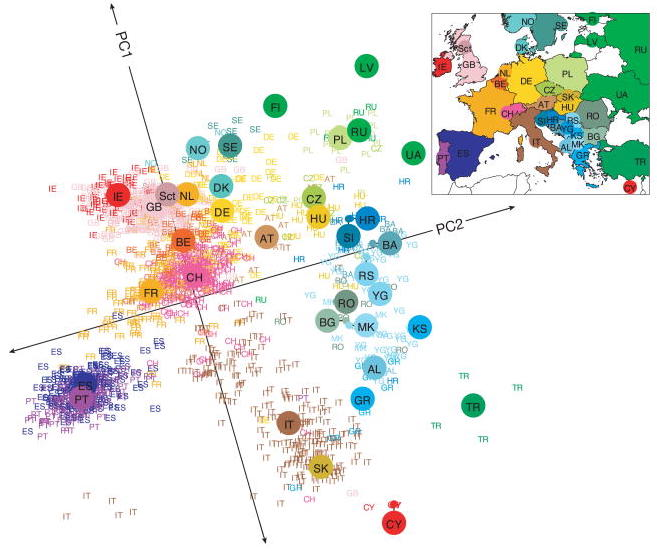
\includegraphics[width=0.95\textwidth]{img/genomemap}	
\end{minipage}\begin{minipage}{8cm}
\textcolor{SeaGreen}{Dimensionality reduction:} compress high-dimensional data into a few directions that preserve most variability.\\[3mm]
\textcolor{SeaGreen}{Noise filtering:} small eigenvalues $\to$ directions with little signal.\\[3mm]
	\textcolor{SeaGreen}{Visualization:} projecting onto first 2 PCs often reveals hidden structure.\\[3mm]
	\textcolor{SeaGreen}{Nice example:} genetic variation in Europeans — plotting individuals on the first two PCs of SNP data \textit{recovers the geographic map of Europe}!  
\end{minipage}
\end{frame}


\begin{frame}{Numerical toy example}
\begin{small}
Covariance matrix:
\[
S=
\begin{pmatrix}
72.9&87.5&6.875\\
87.5&108.3&8.75\\
6.875&8.75&0.73
\end{pmatrix}.
\]

Spectral decomposition:
\[
S = U \Lambda U^\top, \quad
\Lambda=\mathrm{diag}(180,\ 1.38,\ 0.005).
\]

$\Rightarrow$ The first component explains $>99\%$ of the variance; the last can be safely ignored.  
\end{small}
\end{frame}


\begin{frame}{PCA \& Unique football styles}
``\textit{Mille viae ducunt Barcinonem}''\\ 
(A thousand roads lead to Barcelona)\\[3mm]

\begin{minipage}{7cm}
	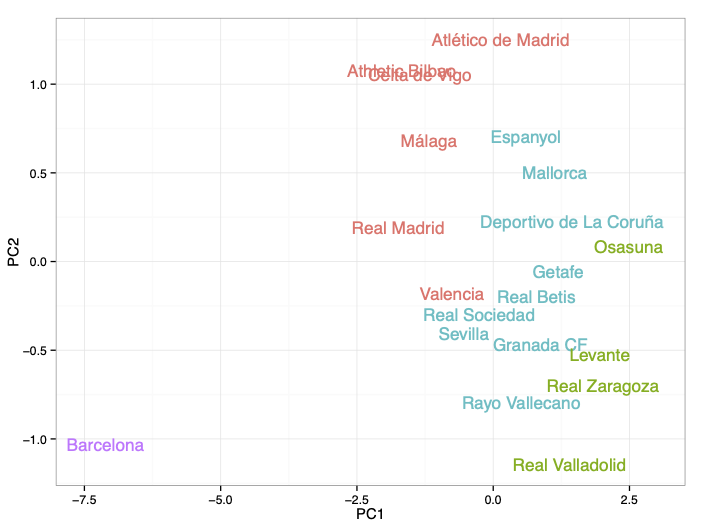
\includegraphics[width=\textwidth]{img/tikitaka}
\end{minipage}
\begin{minipage}{8cm}
	``Searching for a Unique Style in Soccer'' (Gyarmati, Kwak \& Rodriguez, 2014), studies sequential pass patterns in a team's passing.\\[3mm]
They defined ``flow motifs'' as statically significant pass subsequences (e.g., $A\to B\to C\to A$).\\[3mm]
Applied motif analysis to compare styles across teams and leagues. The data are projected to the first two principal components.
\end{minipage}
\end{frame}


\begin{frame}{Quadratic forms}
A \textcolor{SeaGreen}{quadratic form} is $Q({\bf x})={\bf x}^\top  A{\bf x}=\sum_{i,j=1}^n a_{ij}x_ix_j$ with $A\in\R^{n\times n}$ symmetric.
\vskip 6pt
\textcolor{SeaGreen}{Remark:} Since the coefficient of $x_ix_j$ is $a_{ij}+a_{ji}$, every quadratic form has a unique symmetric representative (replace $A$ by $\tfrac{1}{2}(A+A^\top )$).
\vskip 6pt
\textcolor{SeaGreen}{Example:}
\(
\begin{pmatrix}1&2\\ 3&4\end{pmatrix}
\)
and
\(
\begin{pmatrix}1&5/2\\ 5/2&4\end{pmatrix}
\)
define the same $Q(x,y)=x^2+5xy+4y^2$.
 
\end{frame}

\begin{frame}{Signs of quadratic forms}
 
For symmetric $A$:
\begin{enumerate}
\item \textcolor{SeaGreen}{Positive definite}: ${\bf x}^\top  A{\bf x}>0$ for all ${\bf x}\ne{\bf 0}$.
\item \textcolor{SeaGreen}{Negative definite}: ${\bf x}^\top  A{\bf x}<0$ for all ${\bf x}\ne{\bf 0}$.
\item \textcolor{SeaGreen}{Positive semidefinite}: ${\bf x}^\top  A{\bf x}\ge 0$ for all ${\bf x}$.
\item \textcolor{SeaGreen}{Negative semidefinite}: ${\bf x}^\top  A{\bf x}\le 0$ for all ${\bf x}$.
\item \textcolor{SeaGreen}{Indefinite}: takes both positive and negative values.
\end{enumerate}
\textcolor{SeaGreen}{Example:}
\[
{\bf x}^\top 
\begin{pmatrix}1&-1\\ -1&1\end{pmatrix}
{\bf x}=(x-y)^2\ge 0
\]
so the matrix is positive semidefinite.
 
\end{frame}

\begin{frame}{Eigenvalue and minor tests}
 
\textcolor{SeaGreen}{Spectral test (symmetric $A$):}
\begin{itemize}
\item PD $\Longleftrightarrow$ all eigenvalues $>0$;\quad ND $\Longleftrightarrow$ all $<0$;
\item PSD $\Longleftrightarrow$ all $\ge 0$;\quad NSD $\Longleftrightarrow$ all $\le 0$;
\item Indefinite $\Longleftrightarrow$ eigenvalues of different signs.
\end{itemize}
\textcolor{SeaGreen}{Sylvester’s criterion (leading principal minors $D_k$):}
\begin{itemize}
\item PD $\Longleftrightarrow$ $D_k>0$ for $k=1,\ldots,n$;
\item ND $\Longleftrightarrow$ $(-1)^kD_k>0$ for $k=1,\ldots,n$.
\end{itemize}
\textcolor{SeaGreen}{Example:}
\(
A=\begin{pmatrix}-3&2&0\\ 2&-3&0\\ 0&0&-5\end{pmatrix}
\)
has $D_1=-3$, $D_2=5$, $D_3=-25$ $\Rightarrow$ negative definite.
 
\end{frame}

\begin{frame}{Examples}
 
\begin{enumerate}
\item
$
A=\begin{pmatrix}1&4&6\\ 4&2&1\\ 6&1&6\end{pmatrix}
$:
$D_1=1$, $D_2=-14$, $D_3=-109$ $\Rightarrow$ \textcolor{SeaGreen}{indefinite}.
\item
$
A=\begin{pmatrix}3&-1&0\\ -1&2&-1\\ 0&-1&3\end{pmatrix}
$:
$D_1=3$, $D_2=5$, $D_3=12$ $\Rightarrow$ \textcolor{SeaGreen}{positive definite}.
\item The symmetric matrix of $Q(x,y,z)=xy+yz$ is indefinite since $D_1=D_3=0$ and $D_2=-\tfrac14$.
\end{enumerate}
 
\end{frame}


\end{document}